\documentclass[aspectratio=169]{beamer}
\def\mathfamilydefault{\rmdefault}
\usepackage[heading]{ctex}
\usepackage{subfigure,color,bm}
\usepackage{mathtools}
\usepackage{multicol}
\usepackage{minted}
\usepackage{tikz}
\usetikzlibrary{tikzmark}
\usetikzlibrary{arrows.meta}
\usetheme{berlin}

\expandafter\def\expandafter\insertshorttitle\expandafter{%
    \insertshorttitle\hfill%
    \insertframenumber\,/\,\inserttotalframenumber\hfill}

\title{GPU 上的中微子探测}
\author{Berrysoft(王宇逸)}
\institute{清华大学工程物理系}
\begin{document}
\begin{frame}
    \titlepage
\end{frame}
\section{物理背景}
\subsection{基础介绍}
\begin{frame}
    \frametitle{何为中微子}

    \begin{multicols}{2}
        在一个典型的$\beta$衰变中,原子核放出一个电子。
        这个电子的能量服从右图的分布。

        由于能量动量守恒,泡利假设存在另一种粒子分走了部分能量动量。
        费米将其命名为\textbf{中微子}(neutrino)。

        \begin{equation*}
            n\to p+e^-+\bar{\nu}_e
        \end{equation*}
        \columnbreak
        \begin{figure}
            \centering
            \includegraphics[width=0.45\textwidth]{RaE1.jpg}
            \caption{图片来源:维基百科}
        \end{figure}
    \end{multicols}

\end{frame}

\begin{frame}
    \frametitle{江门中微子实验(JUNO)}

    \begin{multicols}{2}
        \begin{figure}
            \centering
            \includegraphics[height=0.6\textheight]{juno_geo.png}
            \caption{JUNO 的地理位置}
        \end{figure}
        \columnbreak
        \begin{figure}
            \centering
            \includegraphics[height=0.55\textheight]{juno_det.png}
            \caption{JUNO 的探测器结构}
        \end{figure}
    \end{multicols}

\end{frame}

\begin{frame}
    \frametitle{JUNO 的物理目标}

    \begin{multicols}{2}
        中微子振荡的发现确认了中微子存在质量,这是一个超出现有标准模型的结论。
        确定三个质量本征态的质量顺序,能够帮助我们排除一些物理模型。

        如今我们能够确定$m_2>m_1,\Delta m_{31}^2 \gg \Delta m_{21}^2$。
        因此中微子质量仅存在两种排序可能:
        $m_3>m_2>m_1$(正序)或$m_2>m_1>m_3$(反序)。

        电子反中微子$\bar{\nu}_e$的能谱根据中微子质量顺序的不同而有着微弱的差异,如右图。
        \columnbreak
        \begin{figure}
            \centering
            \includegraphics[width=0.45\textwidth]{nu_energy.png}
        \end{figure}
    \end{multicols}

\end{frame}
\subsection{探测器物理过程}
\begin{frame}
    \frametitle{逆$\beta$衰变}

    液体闪烁体中含有大量的质子,中微子主要和质子反应:
    \begin{equation*}
        \bar{\nu}_e+p\to n+e^+
    \end{equation*}
    产生的正电子会与液闪分子相互作用,产生大量光子。
    正电子会与电子湮灭:
    \begin{equation*}
        e^+ +e^-\to\gamma+\gamma
    \end{equation*}
    放出的$\gamma$主要与电子发生康普顿散射,被散射的电子也会与液闪分子相互作用产生光子。

\end{frame}

\begin{frame}
    \frametitle{光电倍增管}

    \begin{multicols}{2}
        光电倍增管(PMT)是一个信号放大器。
        它利用光电效应,将光子信号转变为单电子信号。
        再将一个电子变成许多电子,从而形成可以观测的波形。

        \begin{figure}
            \centering
            \includegraphics[width=0.3\textwidth]{pmt_work.png}
            \caption{PMT 的放大原理示意图}
        \end{figure}
        \columnbreak
        \begin{figure}
            \centering
            \includegraphics[height=0.7\textheight]{pmt.jpg}
        \end{figure}
    \end{multicols}

\end{frame}
\section{波形分析}
\subsection{框架}
\begin{frame}{光电子的泊松过程}
    光电子击中 PMT 的过程是一个泊松过程。下图是发光曲线与波形。
    \begin{figure}
        \includegraphics[width=0.8\textwidth]{poissonprocess.2.pdf}
    \end{figure}
    重建算法需要光强$\mu$与发光曲线的时间偏移$t_0$。
\end{frame}

\subsection{FSMP}
\begin{frame}{Fast Stochastic Matching Pursuit (FSMP)}
    我们使用马尔科夫链蒙特卡罗(MCMC)采样这一过程:
    \vspace{8pt}
    \begin{equation}
        p(\tikzmarknode{w}{w}|\tikzmarknode{mu}{\mu})=\sum_{\bm{z},t_0}p(w|\bm{z},t_0)q(\bm{z},t_0)\frac{p(\tikzmarknode{z}{\bm{z}},\tikzmarknode{t}{t_0}|\mu)}{q(\bm{z},t_0)}\tikzmarknode{mcmc}{\approx} C \frac{1}{M}\sum_{i=1}^M\frac{p(\bm{z}_i|t_{0i},\mu)}{p(\bm{z}_i|t_{0i},\mu_0)}
    \end{equation}
    \begin{tikzpicture}[overlay,remember picture,blue,>=Stealth]
        \draw[<-] (w) |- (1,2) node[anchor=south west] {波形};
        \draw[<-] (mu) |- (4,2) node[anchor=south east] {光强};
        \draw[<-] (z) |- (5,2) node[anchor=south west] {光电子序列};
        \draw[<-] (t) |- (10,2) node[anchor=south east] {时间偏移};
        \draw[<-] (mcmc) |- (11,0) node[anchor=south east] {MCMC};
    \end{tikzpicture}
    并估计$t_0$与$\mu$:
    \begin{equation}
        \begin{aligned}
            \hat{t}_0 & =\frac{1}{M}\sum_{i=1}^M t_{0i}     \\
            \hat{\mu} & =\arg\underset{\mu}{\min} ~p(w|\mu)
        \end{aligned}
    \end{equation}
\end{frame}

\begin{frame}{MCMC 的步骤}
    \begin{figure}
        \centering
        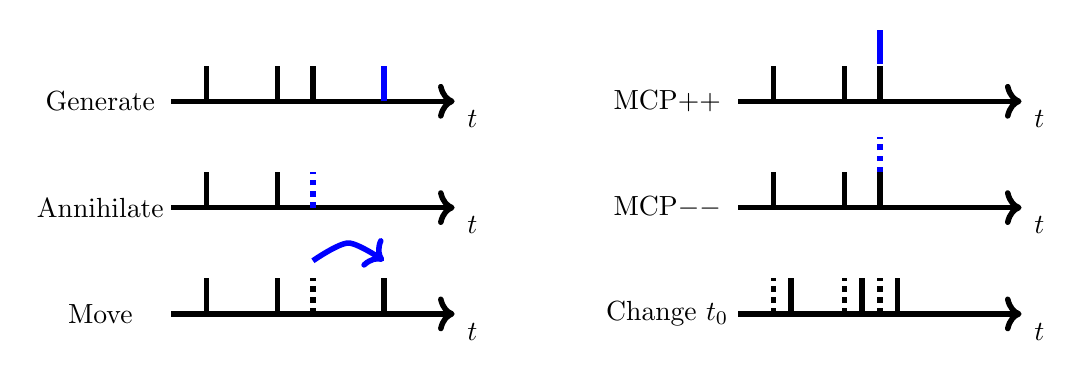
\begin{tikzpicture}[scale=0.45]
            \node[] at (-18,0) {Generate};
            \draw[->,line width=2pt] (-16,0) -- (-8,0);
            \draw[black,line width=2pt] (-15,0) -- (-15,1);
            \draw[black,line width=2pt] (-13,0) -- (-13,1);
            \draw[black,line width=2pt] (-12,0) -- (-12,1);
            \draw[blue,line width=2pt] (-10,0) -- (-10,1);
            \node[] at (-7.5,-0.5) {$t$};

            \node[] at (-18,-3) {Annihilate};
            \draw[->,line width=2pt] (-16,-3) -- (-8,-3);
            \draw[black,line width=2pt] (-15,-3) -- (-15,-2);
            \draw[black,line width=2pt] (-13,-3) -- (-13,-2);
            \draw[dotted,blue,line width=2pt] (-12,-3) -- (-12,-2);
            \node[] at (-7.5,-3.5) {$t$};

            \node[] at (-18,-6) {Move};
            \draw[->,line width=2pt] (-16,-6) -- (-8,-6);
            \draw[black,line width=2pt] (-15,-6) -- (-15,-5);
            \draw[black,line width=2pt] (-13,-6) -- (-13,-5);
            \draw[dotted,black,line width=2pt] (-12,-6) -- (-12,-5);
            \draw[black,line width=2pt] (-10,-6) -- (-10,-5);
            \draw[->,blue,line width=2pt] plot [smooth] coordinates {(-12,-4.5) (-11,-4) (-10,-4.5)};
            \node[] at (-7.5,-6.5) {$t$};

            \node[] at (-2,0) {MCP$++$};
            \draw[->,line width=2pt] (0,0) -- (8,0);
            \draw[black,line width=2pt] (1,0) -- (1,1);
            \draw[black,line width=2pt] (3,0) -- (3,1);
            \draw[black,line width=2pt] (4,0) -- (4,1);
            \draw[blue,line width=2pt] (4,1.05) -- (4,2);
            \node[] at (8.5,-0.5) {$t$};

            \node[] at (-2,-3) {MCP$--$};
            \draw[->,line width=2pt] (0,-3) -- (8,-3);
            \draw[black,line width=2pt] (1,-3) -- (1,-2);
            \draw[black,line width=2pt] (3,-3) -- (3,-2);
            \draw[black,line width=2pt] (4,-3) -- (4,-2);
            \draw[dotted,blue,line width=2pt] (4,-2) -- (4,-1);
            \node[] at (8.5,-3.5) {$t$};

            \node[] at (-2,-6) {Change $t_0$};
            \draw[->,line width=2pt] (0,-6) -- (8,-6);
            \draw[dotted,black,line width=2pt] (1,-6) -- (1,-5);
            \draw[black,line width=2pt] (1.5,-6) -- (1.5,-5);
            \draw[dotted,black,line width=2pt] (3,-6) -- (3,-5);
            \draw[black,line width=2pt] (3.5,-6) -- (3.5,-5);
            \draw[dotted,black,line width=2pt] (4,-6) -- (4,-5);
            \draw[black,line width=2pt] (4.5,-6) -- (4.5,-5);
            \node[] at (8.5,-6.5) {$t$};
        \end{tikzpicture}
    \end{figure}
    这些操作需要满足一定的接受率才会被接受,例如$\displaystyle\min\left\{1, \frac{p(t'_0|\bm{z}_i,\mu)g(t'_0\to t_0)}{p(t_0|\bm{z}_i,\mu)g(t_0\to t'_0)}\right\}$
\end{frame}

\begin{frame}
    \frametitle{收敛性}

    使用 Gelman 和 Rubin 的方法(1992)可以计算混合 MCMC 的收敛性。

    通常,这个链会在 $3000\sim 5000$ 步左右收敛。

    \begin{figure}
        \centering
        \includegraphics[width=0.45\textwidth]{conv.pdf}
    \end{figure}

\end{frame}
\section{GPU 加速}
\subsection{批量处理}
\begin{frame}
    \frametitle{手写 CUDA(失败)}

    \begin{multicols}{2}
        尝试令一个 block 处理一个波形,由于 CUDA 的同步机制,
        恰好可以实现对波形的并行处理。

        我们写了1350行 CUDA 代码(包括单元测试),但是很不幸,
        由于对同步机制的理解并不深刻,代码至今没有跑通。

        但是这些代码\textbf{非常壮观},因此在这里给一点样例。
        \columnbreak
        \begin{figure}
            \includegraphics[height=0.7\textheight]{tsmp.png}
        \end{figure}
    \end{multicols}

\end{frame}

\begin{frame}[allowframebreaks]
    \frametitle{批量处理}

    \begin{figure}
        \centering
        \includegraphics[height=0.7\textheight]{batched1.png}
    \end{figure}

    \begin{figure}
        \centering
        \includegraphics[height=0.7\textheight]{batched2.png}
    \end{figure}

    在 A100 上,可以达到 10ms/波形。

\end{frame}

\subsection{Benchmarks}
\begin{frame}[allowframebreaks,fragile]
    \frametitle{CuPy 与 Tensorflow 的速度对比}

    \begin{figure}
        \centering
        \includegraphics[height=0.75\textheight]{bench.pdf}
    \end{figure}

    \begin{table}
        \centering
        \begin{tabular}{|c|c|}
            CuPy & Tensorflow \\
            \hline
            \begin{minipage}[t]{0.5\textwidth}
                \begin{minted}{python}
sel_add = cp.ElementwiseKernel(
    "float32 delta, bool sel",
    "float32 dest",
    "if(sel) dest += delta",
    "sel_add"
)
def cp_inplace_add(a, b, c):
    sel_add(c, b, a)
                \end{minted}
            \end{minipage}
                 &
            \begin{minipage}[t]{0.5\textwidth}
                \begin{minted}{python}






def tf_inplace_add(a, b, c):
    a = tf.where(b, a + c, a)
                \end{minted}
            \end{minipage}
        \end{tabular}
        \caption{并不知道 Tensorflow 有没有什么高效的 inplace/masked add 方法}
    \end{table}

\end{frame}
\section{结束}
\begin{frame}

    \begin{block}{致谢}
        \begin{itemize}
            \item 续本达(@heroxbd)老师贡献了大量的代码与优化。
            \item 徐大成(@thexdc)同学的波形分析论文:\href{https://arxiv.org/abs/2112.06913}{arXiv:2112.06913}
            \item 杰哥(@jiegec)的多次讨论与 GPU 计算方面的指导。
            \item 哈利教教写 CUDA!
            \item 感谢其他提供点子的同学!
            \item 部分图片来源杂糅,无法完全表明出处。
        \end{itemize}
    \end{block}

    \begin{block}{资源}
        \begin{itemize}
            \item \href{https://github.com/Berrysoft/NeutrinoFSMP}{NeutrinoFSMP}:讲稿,与 benchmark。
            \item \href{https://github.com/Berrysoft/TurboSMP}{TurboSMP}:失败的 CUDA 尝试。
        \end{itemize}
    \end{block}

\end{frame}

\begin{frame}[noframenumbering]

    \begin{minipage}{1\textwidth}
        \centering Q\&A
    \end{minipage}

\end{frame}
\end{document}
